\documentclass[tikz,border=3mm]{standalone}
\usetikzlibrary{positioning,arrows.meta,quotes,decorations.pathmorphing, calc}

\begin{document}
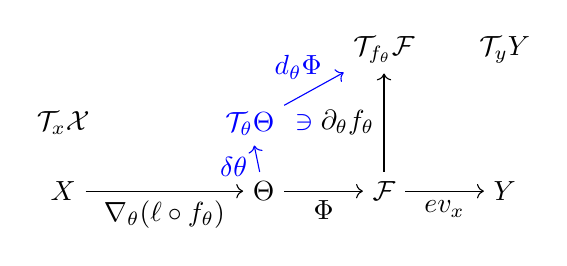
\begin{tikzpicture}[scale=1.0]
\node (X) at (0,0) {$X$};
\node (Theta) [right=2cm of X] {$\Theta$};
\node (F) [right=1cm of Theta] {$\mathcal{F}$};
\node (Y) [right=1cm of F] {$Y$};
\node (TX) [above=0.35cm of X] {$\mathcal{T}_{x} \mathcal{X}$};
\node (TTheta) [left=1cm of F, yshift=0.85cm, blue] {$\mathcal{T}_{\theta} \Theta$};
\node (TF) [above=1.25cm of F] {$\mathcal{T}_{f_{\theta}} \mathcal{F}$};
\node (TY) [above=1.25cm of Y] {$\mathcal{T}_{y} Y$};
\draw[->] (X) to node[below] {$\nabla_{\theta} (\ell \circ f_{\theta})$} (Theta);
\draw[->] (Theta) to node[below] {$\Phi$} (F);
\draw[->, blue] (TTheta) to node[above=0.00cm, xshift=-0.2cm] {$d_{\theta} \Phi$} (TF);
\draw[->, blue] (Theta) to node[left, blue] [yshift=-0.1cm] {$\delta \theta$} (TTheta);
\draw[->] (F) to node[left] {${\color{blue}{\ni}} \; \partial_{\theta} f_{\theta}$} (TF);
\draw[->] (F) to node[below] {$ev_x$} (Y);
\end{tikzpicture}

\end{document}